\subsection{Interval Analysis}\label{sec:interval_analysis}

Nugget uses LLVM passes to automatically annotate programs at the LLVM IR level, enabling interval analysis to be performed directly on real hardware.
Interval analysis is necessary to discover and profile all intervals in a program's execution as defined by the chosen unit of work.
However, profiling an entire program can be time-consuming if done via simulation or emulation (Section~\ref{sec:finding_samples_is_expensive}).

While tools that rely on dynamic instrumentation and binary translation exist to perform such analyses, they often impose restrictions on the ISA and the host platform.
By embedding interval analysis directly into the program's execution, Nugget achieves near-native speed without introducing hardware-specific constraints: any machine capable of running the program can execute the interval analysis.

Because our unit of work is defined at the LLVM IR level and is independent of the final binary, all discovered intervals remain consistent regardless of the host machine's ISA or micro-architecture.
For example, we can analyze a program on an x86 system and then use the resulting intervals to drive sampling on an \revision{Arm} system.

In this section, we describe (1) how Nugget uses LLVM passes to generate an interval analysis executable, and (2) how this executable is used to discover and profile intervals.

\subsubsection{Interval Analysis LLVM Pass}\label{sec:interval_analysis_llvm_pass}

% \begin{figure}[t]
%     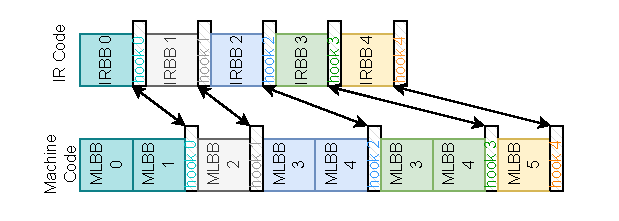
\includegraphics[width=\columnwidth]{images/nugget-hook.pdf}
%     \caption{The interval analysis LLVM pass automatically places a hook at the end of each LLVM IR basic block, so machine-level basic blocks in any final compiled binary are mapped to their LLVM IR basic blocks without any manual calculation.}
%     \label{fig:nugget_hook}
% \end{figure}

The interval analysis LLVM pass, a modular compiler transformation that operates directly on LLVM IR, identifies all basic blocks (IRBBs) in the program's IR.
% For each IRBB, it records the number of LLVM IR instructions and inserts a hook at the end of the block, as illustrated in Figure~\ref{fig:nugget_hook}.
For each IRBB, it records the number of LLVM IR instructions and inserts a hook at the end of the block.
Each hook is uniquely associated with its IRBB and encodes both the block's ID and instruction count, allowing us to retrieve LLVM IR-level information during binary execution.

The hook is a lightweight function that counts occurrences and invokes other functions when specified conditions are met.
This design allows us to flexibly adjust what data to collect by simply changing the functions the hook calls.
After compilation with this LLVM interval analysis pass, the resulting binary executes the hook every time an IRBB is completed, enabling runtime data collection at the LLVM IRBB level.
This hook-based approach also lets us automatically map LLVM IR basic blocks to their corresponding machine-level basic blocks.
We discuss the overheads introduced by the hooks in Section~\ref{sec:overhead_of_hooks}.

\subsubsection{Interval Analysis Executable}\label{sec:interval_analysis_executable}

The interval analysis process has two main goals: (1) to partition the program's execution into a sequence of intervals, and (2) to generate a characteristic signature (e.g., a basic block vector) for each interval.
In Nugget, an interval is defined by a fixed number of executed LLVM IR instructions (Section~\ref{sec:unit_of_work}).
Thus, discovering intervals involves recording the current execution point whenever the LLVM IR instruction count is reached and marking the current execution point as the end of a newly identified interval.

Once intervals are identified, each is characterized by a signature.
Whereas the interval's definition specifies its location in the program's execution, the signature captures its behavioral characteristics.
For example, SimPoint defines intervals by instruction count but represents each interval's signature as a basic block vector that tracks how often each basic block is executed.

A signature is closely tied to the chosen sample selection algorithm.
Since this paper does not propose a new selection algorithm, we do not introduce a new signature.
However, we demonstrate how our hook-based approach can flexibly collect different types of signatures by constructing both LLVM IRBB vectors and count stamp vectors.
The LLVM IRBB vector tracks the frequency of entering each IRBB, while the count stamp vector records the global IR instruction counter value when each IRBB is last entered.
These will later be used to create markers (Section~\ref{sec:nugget_creation}).

\paragraph*{Discovering Intervals}

Discovering intervals is managed by the hooks.
Each hook knows the ID and instruction count of its IRBB.
Whenever a hook executes, it increments a global IR instruction counter by the IRBB's instruction count and checks whether this counter has reached the defined interval size.
If so, a new interval is marked by assigning it a sequential ID; otherwise, execution continues as normal.

All discovered intervals are binary independent because their definitions rely on the LLVM IR-level.
Thus, regardless of the ISA or microarchitecture of the machine running the interval analysis executable, the discovered intervals remain consistent for the final compiled binary.

\paragraph*{Generate A Characteristic Signature}

Our hook-based design makes it easy to specify what data to collect during execution by simply modifying the functions called by each hook.
Because each hook has access to the LLVM IR basic block (IRBB) information, we can build an \emph{IRBB vector} by incrementing a global vector based on the IRBB ID whenever a block is entered.
This vector effectively records how many times each IRBB is executed within an interval, capturing the frequency profile of the program's control flow.
It is recorded and reset whenever a new interval is detected.
Since the LLVM IR control flow remains consistent across all final binaries (Section~\ref{sec:initial_setup}), the IRBB vector is inherently binary independent.

In contrast, the \emph{count-stamp vector} records the global IR instruction count each time an IRBB is entered, marking when during the program's execution each IRBB was last encountered.
This provides a timestamped trace of the control flow relative to instruction execution.
The count-stamp vector is also recorded and reset at the end of each interval.

In Section~\ref{sec:markers}, we show how the IRBB vector is used to create execution markers and how the count-stamp vector helps reduce the hook overhead.
This flexible design allows researchers to explore additional signatures for sampling methodologies with minimal development effort.
